\documentclass{tufte-handout}

\newcommand{\myroot}{../..}
\usepackage[handout]{\myroot/course}
\title{\usnaCourseNumber\ Task 3.2 -- Computer vision: image processing}
\author{\usnaInstructorShort}
\date{\printdate{\courseWeekTwo}}

\usepackage{tikz}
\tikzset{
block/.style={rectangle, minimum width=1.25in, minimum height=3em, text centered, align=center, draw=black, fill=blue!30},
arrow/.style={thick,->,>=stealth},
noarrow/.style={thick}}

\begin{document}
\maketitle
Digital images must be processed to generate actionable information for an algorithm. For this project, we need to identify and track a target with known color and shape in a cluttered environment.

\section{Algorithm overview}
A simplified functional block diagram for the recommended target identification and tracking algorithm is shown in \fref{fig:1}.

\begin{figure}
\begin{center}
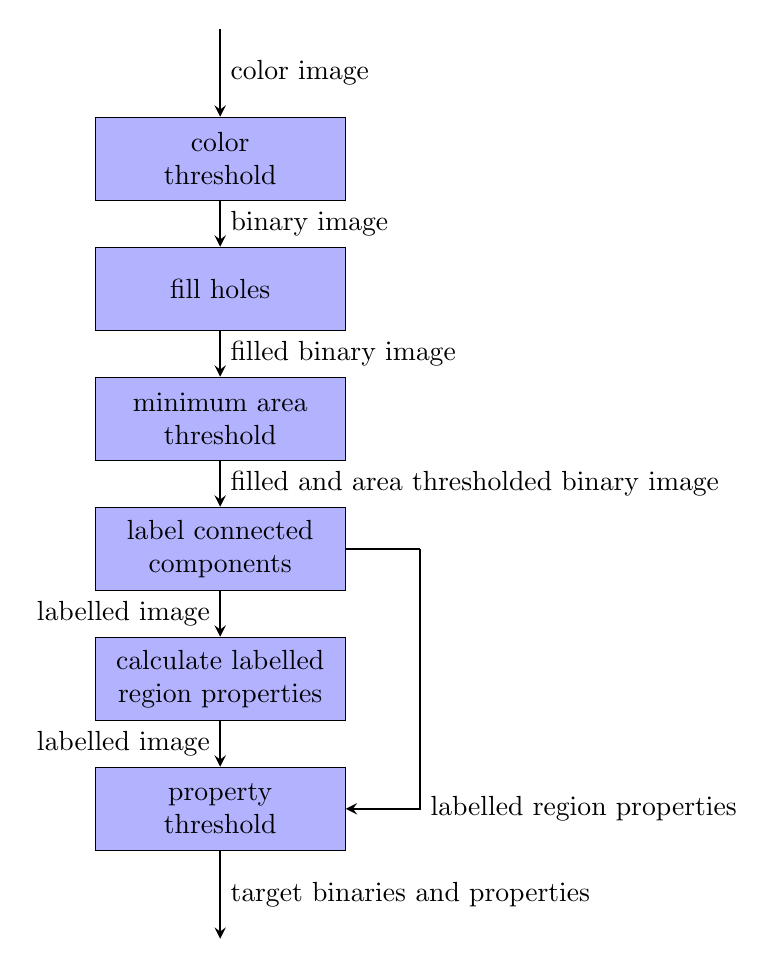
\begin{tikzpicture}
\coordinate (input); 
\node (threshold) [block,below of=input, node distance=0.65in] {color\\threshold};
\node (holes) [block,below of=threshold, node distance=0.65in] {fill holes};
\node (minarea) [block,below of=holes, node distance=0.65in]{minimum area\\threshold};
\node (label) [block,below of=minarea, node distance=0.65in]{label connected\\components};
\coordinate [right of=label, node distance=1in] (llabel);
\node (props) [block, below of=label, node distance=0.65in]{calculate labelled\\region properties};
\node (propthreshold) [block, below of=props, node distance=0.65in]{property\\threshold};
\coordinate [below of=propthreshold, node distance=0.65in] (output);

\draw [arrow] (input) -- node [pos=0.5, right] {color image} (threshold);
\draw [arrow] (threshold) -- node [pos=0.5, right] {binary image} (holes);
\draw [arrow] (holes) -- node [pos=0.5, right] {filled binary image}(minarea);
\draw [arrow] (minarea) -- node[pos=0.5, right] {filled and area thresholded binary image} (label);
\draw [arrow] (label) -- node [pos=0.5, left]{labelled image} (props);
\draw [noarrow] (label) -- (llabel);
\draw [arrow] (llabel) |- node[pos=0.5,right]{labelled region properties} (propthreshold);
\draw [arrow] (props) -- node [pos=0.5, left]{labelled image}(propthreshold);
\draw [arrow] (propthreshold) -- node[pos=0.5, right]{target binaries and properties}(output);
\end{tikzpicture}
\end{center}
\caption{Simplified functional block diagram for the target identification and tracking algorithm.}
\label{fig:1}
\end{figure}

\section{Color thresholding}
The simplest method to isolate objects in an image is using color thresholding techniques. These techniques define a bounding region in color space and keep pixels whose colors fall in that region. Generally, given an $M \times N \times 3$ color image, the outputs of a color thresholding function will be:
\begin{enumerate}
\item An $M \times N$ \textbf{binary image} containing a 1 (i.e. ``true'' value) in pixel locations where the color falls within the bounding region, and a 0 (i.e. ``false'' value) everywhere else.
\item An $M \times N \times 3$ \textbf{masked image} containing the original pixel color values in pixel locations where the color falls within the bounding region, and a designated (typically black or $[0,0,0]$) pixel color values everywhere else.
\end{enumerate}
The binary image output will be largely used in this project, while the masked image may be useful for debugging. 

\section{Creating a color thresholding function}
In the interest of time, we will use the \Matlab\ Color Thresholder App to define our bounding region and create a thresholding function. Given an image contained in the variable \lstinline{im}, the Color Thresholder App can be called using:
\begin{lstlisting}[style=usnaMatlab]
colorThresholder(im);
\end{lstlisting}
This will open a window containing your image and point clouds of four color space options that can be used for thresholding the image (\fref{fig:2}). 
\begin{figure}
\begin{center}
\includegraphics[width=\columnwidth]{\myroot/figures/lab32-f2.png}
\end{center}
\caption{Color space selection prompt associated with the \Matlab\ Color Thresholder App.}
\label{fig:2}
\end{figure}

Per the prompt in the window, each point cloud in 3D color space can be rotated to find the option that best isolates whatever color(s) you want to threshold. Once a viable option is identified, select the color space using the button above the 3D plot. Doing so will update the window based on your selection (\fref{fig:3}). 

\begin{figure}
\begin{center}
\includegraphics[width=\columnwidth]{\myroot/figures/lab32-f3.png}
\end{center}
\caption{Threshold region definition prompt associated with the \Matlab\ Color Thresholder App.}
\label{fig:3}
\end{figure}
The threshold region definition window provides three options to specify a threshold region:
\begin{enumerate}
\item Sketching a region in the image to try and segment (upper left), 
\item Tuning threshold values using sliders for each color channel (upper right), and 
\item\label{method3} Defining a polygon region in rotated 3D color space (lower right). 
\end{enumerate}
While each individual method or combination of methods can be effective, we will focus this effort on method~\ref{method3}. As an example, to threshold the green peppers in the image shown in \fref{fig:3}, we can rotate the color space point cloud to better isolate the green pixels, then draw one or more polygon(s) around those colors in the point cloud (\fref{fig:4}). 

\begin{figure}
\begin{center}
\includegraphics[width=\columnwidth]{\myroot/figures/lab32-f4.png}
\end{center}
\caption{Example of segmenting green peppers by creating two polygon regions in rotated color space using the \Matlab\ Color Thresholder App.}
\label{fig:4}
\end{figure}
As you create closed polygon regions, you will see a masked image form where your original image used to be. The points of each polygon can be adjusted, and polygons can be added/removed until a satisfactory result is achieved. 

Once you are satisfied with your result, you can create your thresholding function by selecting the \lstinline{Export} dropdown and choosing \lstinline{Export Function}. This will automically generate a \Matlab\ function with the default name \lstinline{createMask}. You can choose to adjust this name as needed in the function declaration line of the code, and save the function to your current directory. Be sure the filename matches the function name used in the declaration line of the code. Once saved, you can create a binary image from a color image using:
\begin{lstlisting}[style=usnaMatlab]
bin = createMask(im);
\end{lstlisting}
This assumes that your color image is contained in \lstinline{im} and you kept the default thresholding function name \lstinline{createMask}. In this example, output binary image will be placed in the variable \lstinline{bin}.

\section{Filling holes}
Holes in binary images generated using color thresholding are common. The causes are usually associated with variable lighting and/or reflective surfaces. Holes are defined as black (i.e.  or false) regions that are fully surrounded by white (i.e.  or true) pixels. Assuming a binary image \lstinline{bin}, holes can be removed using the \lstinline{imfill} function in \Matlab\ with the following syntax:
\begin{lstlisting}[style=usnaMatlab]
binFill = imfill(bin,'holes');
\end{lstlisting}
This creates a new binary contained in the variable \lstinline{binFill} with all holes removed.

\section{Minimum area thresholding}
Much like holes, small regions of noise in binary images generated using color thresholding are common. These can be removed by setting a minimum connected component area threshold. Connected components are defined as continuous regions of white pixels, and area is defined by the sum of all connected pixels in a given connected region. Assuming a binary image \lstinline{bin} and a minimum area value of \lstinline{minArea}, minimum area thresholding can be performed using the \lstinline{bwareaopen} function in \Matlab\ with the following syntax:
\begin{lstlisting}[style=usnaMatlab]
binMinArea = bwareaopen(bin,minArea);
\end{lstlisting}
This creates a new binary \lstinline{binMinArea} where regions with areas below the specified \lstinline{minArea} value are removed.

\section{Labelling connected components}
Continuous regions of white pixels (i.e. 1 or true) in a binary image can be separated into individual connected components (i.e. continuous, connected regions of pixels). This is an important tool as individual targets, when properly thresholded, should yield a single connected region of white pixels. 

Assuming a binary image \lstinline{bin}, the connected components can be labelled and the number of connected components can be counted using the \lstinline{bwlabel} function in \Matlab\ with the following syntax:
\begin{lstlisting}[style=usnaMatlab]
[lbl, n] = bwlabel(bin);
\end{lstlisting}
This creates a labelled image \lstinline{lbl} and provides the total number of individual connected components \lstinline{n}. Labelled images contain integer values ranging from 0 to the value contained in \lstinline{n}. The result is an image whose first connected component is filled with 1s, second connected component is filled with 2s, etc. until the $n$th connected component is reached. As with binary images, 0s represent unthresholded regions of the image.

\section{Calculating labelled region properties}
Region properties are measurable attributes associated with a binary region or connected component in a labelled image. While there are numerous properties that can be calculated for a binary or labelled region, we will consider the following subset for this initial investigation: 
\begin{itemize}
\item \textbf{Area} -- the sum or total number of pixels contained in a given binary or labelled region. 
\item \textbf{Centroid} -- the ``center of mass'' associated with a given binary or labelled region. For a target that is symmetric and a single, connected component; we expect the centroid to lie in the middle of the segmented target.
\item \textbf{Eccentricity} -- a measure that quantifies the elongation of a binary or labelled region. Eccentricity values range from 0 (for a perfectly circular region) and 1 (for a region that is a line segment).
\end{itemize}

Given a labelled image \lstinline{lbl}, the region properties of area, centroid, and eccentricity can be calculated for a binary or labelled imaged using the \lstinline{regionprops} command in \Matlab\ with the following syntax:
\begin{lstlisting}[style=usnaMatlab]
stats = regionprops(lbl,'area','centroid','eccentricity');
\end{lstlisting}
This creates an $n$-element structured array \lstinline{stats} (assuming $n$ labelled connected components contained in \lstinline{lbl}) that contains the fields \lstinline{Area}, \lstinline{Centroid}, and \lstinline{Eccentricity}. As an example, the centroid for the second connected component can be recovered using the following syntax:
\begin{lstlisting}[style=usnaMatlab]
cent = stats(2).Centroid;
\end{lstlisting}

\section{Region property thresholding}
Using the properties calculated for the labelled connected component regions of our image, we can eliminate any regions whose properties do not match the properties of known targets. To do this, we can set minimum and maximum threshold values for area and eccentricity. Given:
\begin{itemize}
\item maximum area values for a viable target defined \lstinline{maxArea} and;
\item minimum and maximum eccentricity values for a viable target defined \lstinline{minEcc} and \lstinline{maxEcc},
\end{itemize}
an array of index values \lstinline{idx} of labelled regions whose area and eccentricity value falls within these bounds can be found using the \lstinline{find} command in \Matlab\ with the following syntax:
\begin{lstlisting}[style=usnaMatlab]
idx = find(...
	[stats.Area] <= maxArea & ... 
	[stats.Eccentricity] >= minEcc & ...
	[stats.Eccentricity] <= maxEcc);
\end{lstlisting}
Note that the \lstinline{...} is a line continuation that allows us to separate a single line of code into multiple lines for commenting and better readability. Additionally, minimum area threshold values were imposed previously using \lstinline{bwareaopen}.

Given the index values \lstinline{idx} for regions associated with viable targets, the properties of these regions can be recovered using using the following syntax:
\begin{lstlisting}[style=usnaMatlab]
statsTargets = stats(idx);
\end{lstlisting}
where \lstinline{statsTargets} is a structured array with fields matching \lstinline{stats}. To recover individual binary images of a target, we can use the following:
\begin{lstlisting}[style=usnaMatlab]
for i = idx
	binTargets{i} = lbl == i;
end
\end{lstlisting}
Where \lstinline{binTargets} will be a cell array whose elements are individual binary images.

\section{Packaging your results}
Combine your target thresholding and properties code into a single \Matlab\ function whose input is a color image and whose outputs are properties for viable targets and binaries for each viable target. For example, using the variable names presented in this document:
\begin{lstlisting}[style=usnaMatlab]
[statsTargets,binTargets] = targetThreshold(im);
\end{lstlisting}
this function should accomplish the following:
\begin{enumerate}
\item Clearly define property threshold values (e.g. \lstinline{minArea}, \lstinline{maxArea}, \lstinline{minEcc}, and \lstinline{maxEcc}),
\item Perform color thresholding (using your \lstinline{createMask} or alternately named function),
\item Fill any holes in the resultant binary
\item Impose a minimum area threshold
\item Label connected components
\item Calculate region properties of connected components
\item Impose remaining property thresholding
\item Output target properties and target binaries
\end{enumerate}

\section{Documenting your function}
Take the time to write help documentation for your function. This will be a long semester, and it is easy to forget how to use even code that you have written. The commonly used format for \Matlab\ \lstinline{help} documentation is to prepare a \textbf{docstring} within comments at the start of the function as follows:
\begin{lstlisting}[style=usnaMatlab]
function [out1, out2, ...] = funcName(in1, in2, ...)
%FUNCNAME A brief description of what the function does
%	[out1, ...] = FUNCNAME(in1, ...) an in depth description of how the 
%	function works given the specified input/output combination.
%	Any additional notes/comments/details about the aforementioned function 
%	call.
%
%	[out1, ...] = FUNCNAME(in1, in2, ...) an in depth description of how the 
%	function works given the specified input/output combination.
%	...
%
% 	See also RELATEDFUNC1, RELATEDFUNC2, ...
%
%	Contributor(s) names & date initially created
\end{lstlisting}

\section{Bringing it all together}
Take the time to combine everything you have learned into a single \Matlab\ script to accomplish the following:
\begin{enumerate}
\item Initialize your camera and acquire an image
\item Create a figure named \lstinline{EW309 - Target Threshold Test} (use the \lstinline{Name} property) 
\item Create an axes in your figure and adjust the \lstinline{NextPlot} property
\item Add your image to the axes
\item Add a line object that we can use to display centroids (created using the \lstinline{line} or \lstinline{plot} functions). For example, given an axes object handle \lstinline{axs}, to create a large magenta asterisk: 
\begin{lstlisting}[style=usnaMatlab]
cnt = plot(0,0,'*m','Parent',axs,'MarkerSize',10);
\end{lstlisting}
\item Create an indefinite \lstinline{while} loop (using \lstinline{while true})
\begin{enumerate}
\item Get an updated image
\item Update your image object color data with the new image (use the \lstinline{CData} property)
\item Perform your target thresholding
\item Update your line object with the centroid of the first viable target (use the \lstinline{XData} and \lstinline{YData} property)
\item Allow your plot to update using the \lstinline{drawnow} command
\end{enumerate}
\end{enumerate}

\end{document}